La figura mostra la gràfica d'una funció $f$. La recta discontínua és una asímptota
vertical; els cercles buits indiquen punts que no pertanyen a la gràfica i els cercles
plens, punts que sí que hi pertanyen.

\begin{center}
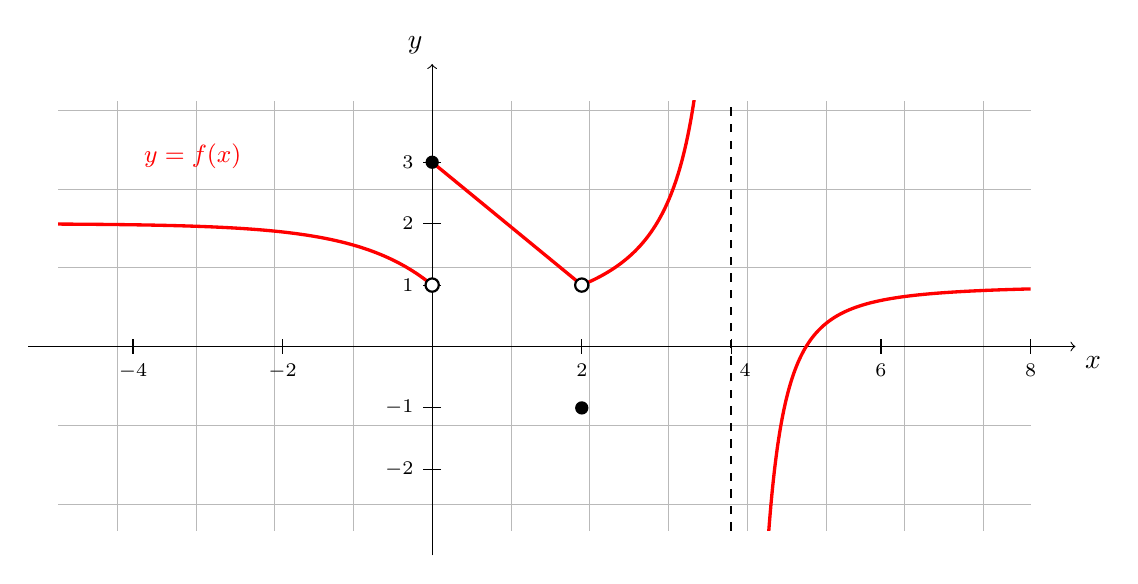
\begin{tikzpicture}[x=0.95cm,y=0.78cm]
  % Branques:  2-e^x  |  recta (0,3)-(2,1)  |  2/(4-x)  |  1-1/(x-4)^2
  \draw[gray!55,very thin] (-5,-3) grid (8,4);
  \draw[->] (-5.4,0) -- (8.6,0) node[below right] {$x$};
  \draw[->] (0,-3.4) -- (0,4.6) node[above left] {$y$};
  \foreach \i in {-4,-2,2,6,8} \draw (\i,0.12) -- (\i,-0.12) node[below,font=\scriptsize] {$\i$};
  \draw (4,0.12) -- (4,-0.12) node[below,xshift=5pt,font=\scriptsize] {$4$};
  \foreach \j in {-2,-1,1,2,3} \draw (0.12,\j) -- (-0.12,\j) node[left,font=\scriptsize] {$\j$};
  \draw[dashed,thick] (4,-3) -- (4,4);
  \begin{scope}
    \clip (-5,-3) rectangle (8,4);
    \draw[red,very thick,domain=-5:0,samples=80,smooth] plot (\x,{2-exp(\x)});
    \draw[red,very thick] (0,3) -- (2,1);
    \draw[red,very thick,domain=2:3.6,samples=80,smooth] plot (\x,{2/(4-\x)});
    \draw[red,very thick,domain=4.4:8,samples=100,smooth] plot (\x,{1-1/((\x-4)^2)});
  \end{scope}
  \draw[fill=white,thick] (0,1) circle (2.4pt);
  \fill (0,3) circle (2.4pt);
  \draw[fill=white,thick] (2,1) circle (2.4pt);
  \fill (2,-1) circle (2.4pt);
  \node[red,font=\small] at (-3.2,3.1) {$y=f(x)$};
\end{tikzpicture}
\end{center}

\begin{apartats}

\apartat{1,25}
A partir de la gràfica, determina el valor dels límits següents. Si algun no existeix,
indica-ho i justifica-ho amb els límits laterals.
\begin{graella}{4}
  \sa \lim_{x\to-\infty}f(x) & \sa \lim_{x\to0^-}f(x) & \sa \lim_{x\to0^+}f(x) & \sa \lim_{x\to2}f(x)\\[10pt]
  \sa \lim_{x\to4^-}f(x) & \sa \lim_{x\to4^+}f(x) & \sa \lim_{x\to+\infty}f(x)
\end{graella}

\begin{solucio}
i) $2$ \quad ii) $1$ \quad iii) $3$ \quad iv) $1$ (els dos laterals valen 1)
\quad v) $+\infty$ \quad vi) $-\infty$ \quad vii) $1$.
\end{solucio}

\apartat{1,25}
Estudia la continuïtat de $f$ en $x=0$, $x=2$ i $x=4$. Si en algun d'aquests punts no és
contínua, classifica'n la discontinuïtat (evitable, de salt finit o de salt infinit) i
justifica-ho amb el valor de la funció i els límits.

\begin{solucio}
$x=0$: $f(0)=3$, però els laterals valen $1$ i $3$. Com que són finits i diferents,
hi ha una \textbf{discontinuïtat de salt finit} (de salt $2$).\\
$x=2$: els dos laterals valen $1$, així que $\lim_{x\to2}f(x)=1$, però $f(2)=-1$.
Com que el límit existeix i no coincideix amb la imatge, la \textbf{discontinuïtat és evitable}.\\
$x=4$: $f(4)$ no existeix i els laterals valen $+\infty$ i $-\infty$.
\textbf{Discontinuïtat de salt infinit} (asímptota vertical $x=4$).
\end{solucio}

\end{apartats}
